% !TeX spellcheck = en_GB

\section{Morphology and Physiology of Individual Neurons}
\label{sec:neurophysiology}

\begin{figure}
	\centering
	{\phantomsubcaption\label{fig:neuron_sketches_motor}}%
	{\phantomsubcaption\label{fig:neuron_sketches_pyramidal}}%
	{\phantomsubcaption\label{fig:neuron_sketches_purkinje}}%
	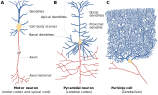
\includegraphics{media/chapters/02_modelling/02_01/neuron_sketches.pdf}
	\caption[Drawings of neurons in different brain regions]{Drawings of neurons in different brain regions.
	Although key structural elements can be identified across neurons, they can have very different morphologies.
	Redrawn from Ramón y Cajal.
	Overall presentation from \citet{kandel2012principles}, Figure~2-3D, p.~25.
	\textbf{(A)} Schematic drawing of a motor neuron (\cite{ramonycajal1894nouvelles}, Figure 6, p.~25).
	\textbf{(B)} Human cortical pyramidal neuron (\cite{howell1916textbook}, Figure~84, p.~187).
	\textbf{(C)} Human purkinje cell in the cerebellum (\cite{ramonycajal1909histologie}, Figure~9, p.~61).
	\label{fig:neuron_sketches}
	}
\end{figure}

Neurons come in various sizes, shapes, and degrees of interconnectedness.
Ramón y Cajal's\index{Ramón y Cajal, Santiago} drawings (schematically redrawn in \Cref{fig:neuron_sketches}) offer a glimpse of the morphological diversity found in the nervous system.
Some neurons possess only few branches (also \emph{projections}\index{neuron!projection}) and have a comparably simple structure, whereas others, such as Cerebellar Purkinje cells, feature sprawling dendritic trees more deserving of the name \enquote{dendritic forest}.

It should come as no surprise that the following review of neural morphology and physiology cannot do justice to the incredible complexity observed in nature.
Our goal is to instead focus on structural and functional elements commonly observed across all neurons.
As a side-effect, the resulting characterisation of the nervous system lends itself well to computational models.
%While the simplifications we make come at the risk of ignoring details that could turn out to be essential for modelling brain function, some simplification
%Yet, as discussed above, we would like to develop theories that bridge as many levels of scale as possible.
%The aspects of biology that we incorporate into our models are known to play a major role in overall brain function.
We open with a high-level overview of neural function and structure, and then focus on aspects of neural electrophysiology that will be relevant in later sections, including the generation of the membrane potential, action potentials, and synaptic transmission.
Readers interested in a more thorough introduction to neuroscience are encouraged to consult neuroscience textbooks such as \citet{bear2016neuroscience}, \citet{purves2017neuroscience}, or \citet{kandel2012principles}.

\subsection{Functional and Structural Overview}
\label{sec:neurons_overview}

\begin{figure}
	\centering
	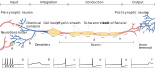
\includegraphics{media/chapters/02_modelling/02_01/neuron_signals_overview.pdf}
	\caption[Overview of neural function]{Overview of neural function. Inset diagrams illustrate the membrane potential over time at the indicated locations (data from a compartmental Hodgkin-Huxley-type model neuron). Arrows indicate the predominant flow of information. \emph{Input:} Neurons receive signals from pre-synaptic neurons through synapses. For chemical synapses, action potentials (\enquote{spikes}) arriving at the synapse (\emph{a}) cause a release of neurotransmitter that induces a post-synaptic potential (PSP) in the post-synaptic neuron (\emph{b}). \emph{Integration:} PSPs from multiple pre-synaptic neurons interact in the dendrites. Under certain conditions the neuron produces its own action potential (\emph{c}). \emph{Conduction:} The action potential travels along the axon (\emph{d}-\emph{e}). \emph{Output:} The neuron induces a PSP in a post-synaptic neuron (\emph{f}).
	}
	\label{fig:neuron_signal_overview}
\end{figure}

From the perspective of computer science---and as suggested by the neuron doctrine---neurons are fundamental units of computation in biological systems.
Specifically, neurons employ weak bioelectric signals, variations in their membrane potential, to compute.
As depicted in the lower portion of \Cref{fig:neuron_signal_overview}, these variations can either be gradual, as is the case when the neuron is in its \emph{subthreshold} regime\index{membrane potential!subthreshold}, or manifest themselves as rapid swings between the highest and lowest voltages that can be produced by a neuron; in this case the neuron is in its \emph{superthreshold} regime.
These rapid voltage changes are called \emph{action potentials}\index{action potential}, or, more colloquially, \enquote{\emph{spikes}}, harking back to their prominent appearance on oscillograms.
% TODO: Index: spike -> action potential

Typically, gradual subthreshold potentials are not directly accessible from other parts of the network;
this analogue code is solely part of a neuron's internal state.
Hence, from the perspective of other neurons in the network, a neuron is either \enquote{silent} or \enquote{spiking}.
This binary nature of neurons fascinated early computer scientists such as \citet{vonneumann1958computer}\index{Von Neumann,John} and led to the development of the first artificial neural networks by \citet{mcculloch1943logical}.

Neuroscientists typically divide neural information processing into four stages: input, integration, conduction, and output \citep[Chapter 2]{kandel2012principles}.
These stages roughly correspond to different features of neural structure, as depicted in \Cref{fig:neuron_signal_overview}.

The \emph{input region} corresponds to the dendrites, and the synapses embedded therein.%
\footnote{
The difference between input and output regions of a neuron is not always clear-cut.
Invertebrate unipolar cells only possess a single branch that protrudes from the cell body.
This branch is referred to as \enquote{axon} although it carries both input and output \citep[Chapter~2]{kandel2012principles}.}
Dendrites are tree-like structures protruding out of the cell body, typically less than two millimetres long \citep[Chapter~1]{bear2016neuroscience}.
They are usually classified according to their location relative to the cell body.
For example, in pyramidal cells (cf.~\Cref{fig:neuron_sketches_pyramidal}) dendrites directly connected to the soma are called \emph{basal}\index{dendrite!basal}; dendrites indirectly connected to the soma through longer projections are called \emph{apical}\index{dendrite!apical}.
Apical dendrites are sometimes additionally divided---using standard anatomical terminology---into parts referred to as \emph{proxmial} or \emph{distal}; that is, they are either closer or father away from the soma \citep[e.g.,][Figure~5]{seamans1997contributions}.

Synapses form the coupling sites between neurons and---in the case of chemical synapses discussed below---establish a unidirectional flow of information.
This ensures that pre-synaptic neurons only influence the state of the post-synaptic neuron, but not vice-versa \citep[Chapter~8]{kandel2012principles}.
Some neurons in the periphery of the nervous system act as sensors; they transduce modalities such as temperature, pressure or light and do not rely on synaptic inputs \citep[Chapter~22]{kandel2012principles}.

The neuron's \emph{integration region} is formed by the cell body and, to some degree, the dendritic tree itself.
Signals from several pre-synaptic neurons interact here.
This interaction may elicit the generation of an output signal.
As we mentioned before, this output takes the form of an \emph{action potential}\index{action potential} in most vertebrate neurons \citep[Chapter~2]{kandel2012principles}.
Crucially, and in contrast to artificial neural networks, the integration process has a temporal component; the input \emph{history} is relevant for the generation of the output, and not just the momentary input.

The \emph{conductive region} corresponds to a neuron's axon\index{axon}.
The axon carries signals generated by the neuron to other parts of the nervous system.
Two features of the axon work in tandem to ensure signal integrity \citep[Chapter~7]{kandel2012principles}.
First, the axon is electrically well insulated, being tightly wrapped in Schwann's cells\index{Schwann's cell}, a type of glial cell\index{glial cell}.
Second, axons actively renew action potentials at Nodes of Ranvier\index{Node of Ranvier}, gaps between neighbouring Schwann's cells.
Conduction is unidirectional in the sense that action potentials only travel away from the origin of excitation.
Notably, in larger animals such as humans, individual neurons conduct signals across micrometres (between neighbouring neurons), centimetres (connecting different parts of the brain), and metres (motor neurons in the spinal cord).%

Finally, the \emph{output region} corresponds to the area surrounding the synapses that lie between the axon terminals and post-synaptic dendrites.
In the case of chemical synapses, the arrival of an action potential at the axon terminal causes the release of neurotransmitter molecules.
Receptors in the post-synaptic neuron transduce neurotransmitters into an input signal, a post-synaptic potential.
In the periphery, axon terminals may be coupled to muscle fibres, where the arrival of an action potential generates movement \citep[Chapter~8~\&~9]{kandel2012principles}.

\subsection{Ion channels and the membrane potential}
\label{sec:membrane_potential}

\begin{figure}
	\centering
	{\phantomsubcaption\label{fig:neuron_membrane_potential_membrane}}%
	{\phantomsubcaption\label{fig:neuron_membrane_potential_membrane_isolated}}%
	{\phantomsubcaption\label{fig:neuron_membrane_potential_membrane_channel}}%
	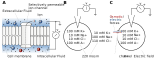
\includegraphics{media/chapters/02_modelling/02_01/neuron_membrane_potential.pdf}
	\caption[Membrane potential as a result of selectively permeable ion channels]{
	Membrane potential as a result of selectively permeable ion channels.
	\textbf{(A)} The cell membrane separates the intra- and extracellular fluid. Charge carriers (e.g., ions) are in solution in the fluids. The membrane potential is the voltage \vMem across the membrane.
	Specific ions may pass through selectively permeable channels.
	\textbf{(B)} If the membrane was a perfect insulator, there would be no membrane potential. Molar concentration in $\mathrm{mM} = \si{\milli\mole\per\litre}$; values illustrative. $A^-$ corresponds to charged anionic molecules.
	The individual fluids are electrically neutral.
	\textbf{(C)} Adding a selectively permeable ion channel results in a membrane potential specific to the ion species at which electric and osmotic forces cancel out.
	Illustrations (B, C) adapted from \citet{reichert2000neurobiologie}, Figures 2.8 and 2.10.}
\end{figure}

As mentioned above, neurons process information by systematically varying their membrane potential\index{membrane potential}\index{potential!membrane} \vMem (more precisely, their \emph{transmembrane} potential).
The membrane potential is the electrical potential between the inside and outside of a cell.
The boundary between these regions is formed by the cell membrane, a double-layer of lipids.%
\footnote{To be clear, \emph{all} biological cells possess bioelectrical properties, including a membrane potential.
This was for example analysed in detail by Julius Bernstein\index{Bernstein, Julius} in the early 1900s \citep{bernstein1912elektrobiologie}. Membrane potentials are important for homeostasis and cell-to-cell communication \citep{moorhouse2016membrane}.
For example, electrical gradients between cells are crucial for laying out the body plan of organisms \citep{levin2014molecular}.
Neurons should be thought of as cells shaped by evolution to excel at bioelectrical signalling, but are not unique in their use of bioelectricity.}
By convention, if the \emph{inside} is more positively charged than the outside, we report a positive voltage (\Cref{fig:neuron_membrane_potential_membrane}).

Measuring the membrane potential when a neuron is at rest---that is, when the cell does not receive any input---reveals the so-called resting potential \vRest.
In mammals, \vRest ranges from \SIrange{-50}{-85}{\milli\volt} depending on the cell type \citep{moorhouse2016membrane}.

Upon closer investigation, the presence of a non-zero resting potential is rather surprising.
The inside and outside of the cell are filled with watery solutions: the intracellular fluid (\enquote{cytoplasm}\index{cytoplasm}) and the extracellular fluid.
Both fluids are electrically neutral.
That is, although the fluids contain ions and anionic charge carriers in solution, the overall positive and negative charges are balanced.
There should be no measurable electrical potential (\Cref{fig:neuron_membrane_potential_membrane_isolated}).


\subsubsection{Selectively permeable ion channels generate the membrane potential}
\begin{figure}
	\centering
	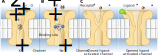
\includegraphics{media/chapters/02_modelling/02_01/channel.pdf}%
	{\phantomsubcaption\label{fig:ion_channels_k}}%
	{\phantomsubcaption\label{fig:ion_channels_na}}%
	{\phantomsubcaption\label{fig:ion_channels_gate}}%
	\caption[Schematic illustration of ion channels  embedded into the cell membrane]{Schematic illustration of ion channels embedded in the cell membrane. Ion channels are pores that selectively let ions of a certain species pass. Selectivity is achieved by exploiting the radius and charge distributions of the ion and its watery hull. \textbf{(A)} Although the $\mathrm{K^+}$ ion is larger than the $\mathrm{Na^+}$ ion, its watery hull is more compact, and it can pass through narrower channels. \textbf{(B)}  $\mathrm{Na^+}$ selectivity is achieved by a negative binding site in the channel that stabilises the $\mathrm{K^+}$ ion and its hull to let it pass.  \textbf{(C)} Ion channels can change their conformation depending on external factors (e.g.~mechanical forces, chemicals, electrical potentials); here, a chemical ligand opens a channel. Inspired by \citet[Figure~5-1, p.~102 and Figure~5-6, p.~109]{kandel2012principles}; see ibid.~for more information.}
\end{figure}
The resting potential can be explained if we assume that the cell membrane is selectively permeable to some ions through so-called \emph{ion channels}\index{ion channel}.
The presence of ion channels has been postulated for a long time, though it is only thanks to relatively recent studies that we understand the molecular machinery that underpins selective permeability \citep[Chapter~5]{kandel2012principles}.

Ion channels are porous proteins embedded in the cell membrane.
They accomplish the impressive feat of acting as an \enquote{atomic sieve}.
This \enquote{sieve} only lets a single ion of a certain kind (in chemical parlance: \emph{ion species}\index{ion species}) pass at a time, as is illustrated in \Cref{fig:ion_channels_k,fig:ion_channels_na}.
Furthermore, as we will see both in the context of action potential generation and synaptic transmission, these proteins can change their shape, or \emph{conformation}, depending on various external circumstances, effectively opening or closing the channel (\Cref{fig:ion_channels_gate}).

Of course, the mere presence of selectively permeable channels does not explain the membrane potential.
For this, we have to consider that despite being electrically neutral, the intra- and extracellular fluids contain different concentrations of the individual charge carriers.
In particular, there are large concentration gradients for potassium ($\mathrm{K^+}$), sodium ($\mathrm{Na^+}$) and chloride ($\mathrm{Cl^-}$) ions.
For example, the concentration of potassium ions $\mathrm{K^+}$ is about \SI{140}{\milli\mol\per\litre} in the cytoplasm, compared to \SI{3}{\milli\mol\per\litre} in the extracellular fluid.
If the cell membrane was permeable to $\mathrm{K}^+$ ions, an osmotic force would act on the ions, driving them outside.

This ionic flow disturbs the charge balance of the intra- and extracellular fluids and results in a non-zero membrane potential.
In turn, this potential results in an electric force that counters the osmotic pressure.
In our $\mathrm{K}^+$ example, the intracellular fluid becomes negatively charged and the ensuing electric attraction reduces the net force acting on the $\mathrm{K}^+$ ions.
The system converges to an equilibrium point where the electric and osmotic forces cancel out (\Cref{fig:neuron_membrane_potential_membrane_channel}).
The membrane potential at this point is called the \emph{equilibrium}\index{equilibrium potential}\index{potential!equilibrium} or \emph{reversal potential}\index{reversal potential}\index{potential!reversal}, as the ionic flow direction reverses at this point.
For clarity, we use the term reversal potential when talking about the equilibrium potential for a membrane permeable to a \emph{single} ion.


\subsubsection{A single selectively permeable ion channel: The Nernst equation}
For a single charge carrier $X$, the reversal potential $E_X$ can be computed using the Nernst equation\index{Nernst equation} \citep{nernst1888kinetik}:%
\footnote{The Nernst equation was published in 1888, before there were established theories about bioelectricity. Nernst studied the electrochemistry of electrolytes separated by membranes and this research was later incorporated into analyses of biological cell membranes by Ostwald and later Bernstein \citep[see][Chapter~5]{bernstein1912elektrobiologie}\index{Bernstein, Julius}.}
\newcommand{\Cout}[1]{\ensuremath{[\mathrm{#1}]_\mathrm{out}}}
\newcommand{\Cin}[1]{\ensuremath{[\mathrm{#1}]_\mathrm{in}}}
\begin{align}
	E_X &= -\frac{RT}{zF} \log \left( \frac{\Cin{X}}{\Cout{X}} \right) \,,
	\label{eqn:nernst}
\end{align}
where $R$ is the gas constant, $T$ is the temperature, $z$ is the charge number, or valence\index{valence}, of the particle (e.g., $z = 2$ for $\mathrm{Ca}^{2+}$ and $-1$ for $\mathrm{Cl}^-$) and $F$ is the Faraday constant. \Cout{X} and \Cin{X} are the concentrations (count per volume) of particles $X$ outside and inside the cell, respectively.
Note that the number of ions flowing through the cell membrane is rather minuscule compared to the total number of ions in solution; \Cout{X} and \Cin{X} essentially do not change over time.%
\footnote{The ion concentrations in the intra- and extracellular fluid are maintained by ion pumps in the cell membrane. These pumps are secondary for a cell's short-term bioelectrical properties, but are indispensible in the long run.}

\begin{table}
	\centering
	\caption[Ion concentrations and reversal potentials in the squid and mammals]{Ion concentrations and reversal potentials in the squid and mammals. Data from \citet[Table~12.1, p.~353]{mccormick2014membrane}. The squid data are based on \citet{hodgkin1949effect}, and reported similarly in \citet[Table~6-1, p.~128]{kandel2012principles}. Reversal potentials computed using \cref{eqn:nernst}.}
	\label{tbl:nernst}
	\small
	\sffamily
	\begin{tabular}{l l p{0.25cm} r r p{0.25cm} r r}
		\toprule
		&
		&
		& \multicolumn{2}{c}{\textbf{Concentrations}}
		&
		& \multicolumn{2}{c}{\textbf{Reversal potentials}} \\ %  \multicolumn{1}{c}{\textbf{Permeability ratios}}\\
		\cmidrule(lr){4-5}\cmidrule(lr){7-8}
		
		\multicolumn{2}{l}{\textbf{Ion species}}
		&
		& \emph{Intracellular}
		& \emph{Extracellular}
		&
		& $T = \SI{20}{\degreeCelsius}$
		& $T = \SI{36}{\degreeCelsius}$ \\ %& $P_\mathrm{K^+} : P_\mathrm{Na^+} : P_\mathrm{Cl^-}$ \\
		\midrule

		\multicolumn{2}{l}{\emph{Squid giant axon}}\\

		\raggedleft \quad Potassium
		& $\mathrm{K}^+$
		&
		& \SI{400}{\milli\mol\per\litre}
		& \SI{20}{\milli\mol\per\litre}
		&
		& \SI{-76}{\milli\volt}
		& \SI{-80}{\milli\volt} \\

		\raggedleft \quad Sodium
		& $\mathrm{Na}^+$
		&
		& \SI{50}{\milli\mol\per\litre}
		& \SI{440}{\milli\mol\per\litre}
		&
		& \SI{55}{\milli\volt}
		& \SI{58}{\milli\volt} \\

		\raggedleft \quad Chloride
		& $\mathrm{Cl}^-$
		&
		& \SI{40}{\milli\mol\per\litre}
		& \SI{560}{\milli\mol\per\litre}
		&
		& \SI{-67}{\milli\volt}
		& \SI{-70}{\milli\volt} \\[0.25cm]

		\multicolumn{2}{l}{\emph{Mammalian neuron}}\\

		\raggedleft \quad Potassium
		& $\mathrm{K}^+$
		&
		& \SI{140}{\milli\mol\per\litre}
		& \SI{3}{\milli\mol\per\litre}
		&
		& \SI{-97}{\milli\volt}
		& \SI{-102}{\milli\volt} \\

		\raggedleft \quad Sodium
		& $\mathrm{Na}^+$
		&
		& \SI{18}{\milli\mol\per\litre}
		& \SI{145}{\milli\mol\per\litre}
		&
		& \SI{53}{\milli\volt}
		& \SI{56}{\milli\volt} \\

		\raggedleft \quad Chloride
		& $\mathrm{Cl}^-$
		&
		& \SI{7}{\milli\mol\per\litre}
		& \SI{120}{\milli\mol\per\litre}
		&
		& \SI{-72}{\milli\volt}
		& \SI{-76}{\milli\volt} \\

		\bottomrule
	\end{tabular}
\end{table}

\subsubsection{Multiple selectively permeable ion channels: The Goldman-Huxley-Katz equation}
\Cref{tbl:nernst} lists the ion concentrations of the squid giant axon---a model system common in the early days of neuroscience---as well as mammalian cells.
Although there are large differences in the ion concentrations, the reversal potentials (when computed using eq.~\ref{eqn:nernst}) are similar across species.
Still, we find that, in general, no individual reversal potential exactly matches the resting potential.
For example, in the squid, the resting potential is close to \SI{-62}{\milli\volt} at a temperature of \SI{20}{\degreeCelsius} (\cite{mccormick2014membrane}).
This potential is slightly more positive than $E_\mathrm{K^+}$ and $E_\mathrm{Cl^-}$, but much more negative than $E_\mathrm{Na^+}$.

This suggests that the cell membrane is permeable to several ion species at the same time, but at different \enquote{permeabilities}.
The membrane potential converges to a new equilibrium state $E$ somewhere between the original reversal potentials.
Mathematically, we summarise the relative permeability of the cell membrane for an ion species $X$ as a quantity $P_X$.
Instructively, $P_X$ can be interpreted as the total number of open ion channels for an ion species $X$.

We can compute the overall equilibrium potential using the Goldman-Huxley-Katz equation\index{Goldman-Huxley-Katz equation} \citep{goldman1943potential,hodgkin1949effect}.
For the three ion species listed above we have
\begin{align}
	E &= \frac{RT}{F} \log \left( \frac{
		P_\mathrm{K^+} \Cout{K^+} +
		P_\mathrm{Na^+} \Cout{Na^+} +
		P_\mathrm{Cl^-} \Cin{Cl^-}}{
		P_\mathrm{K^+} \Cin{K^+} +
		P_\mathrm{Na^+} \Cin{Na^+} +
		P_\mathrm{Cl^-} \Cout{Cl^-}
		} \right) \,.
	\label{eqn:goldman}
\end{align}
For the squid giant axon, the permeability ratios $P_\mathrm{K^+} : P_\mathrm{Na^+} : P_\mathrm{Cl^-}$ can be experimentally determined to be about $1: 0.04 : 0.45$---in its resting state, the membrane is strongly permeable to potassium, but only weakly so for sodium \citep{mccormick2014membrane}.
Plugging these numbers into \cref{eqn:goldman} results in the resting potential $\vRest \approx \SI{-62}{\milli\volt}$.

\subsubsection{Equivalent circuit model}
\begin{figure}
	\centering
	\includegraphics[scale=0.3333]{media/chapters/02_modelling/02_01/electrical_circuit.pdf}
	{\phantomsubcaption\label{fig:electrical_circuit_individual_channels}}
	{\phantomsubcaption\label{fig:electrical_circuit_membrane}}
	\caption[Electrical circuit model of the cell membrane]{Electrical model circuit of the cell membrane.
	\textbf{(A)} Individual ion channels can be modelled as a resistor-voltage-source pair (\emph{left}).
	Instead of modelling all ion channels for the same ion species $X$ independently, they can be mathematically combined into a single pair (\emph{right}).
	\textbf{(B)} Circuit model of a neuron at rest. The ratios of the conductances $g_\mathrm{K^+}$, $g_\mathrm{Na^+}$, and $g_\mathrm{Cl^-}$ determine the cell's equilibrium potential $E$. Arrows indicate the current direction relative to $E = \SI{0}{\volt}$ (not physical ionic flow).}
	\label{fig:electrical_circuit}
\end{figure}
Alternatively, the equilibrium potential can be modelled in terms of the equivalent circuit depicted in \Cref{fig:electrical_circuit}.
The idea is the following.
An ion species $X$ is \enquote{driven} by the voltage difference between the membrane potential \vMem and the reversal potential  $E_X$ (eq.~\ref{eqn:nernst} and \Cref{tbl:nernst}).
Each ion channel provides a conductive path for a specific ion species $X$; however, the channels are tiny, and ionic movement is influenced by thermal Brownian noise.
Hence, there is a chance that ions will collide with the cell interior before passing through a channel.
This provides a resistance $R_X$ to the ionic current \citep{enderle2011bioelectric}.

Each ion channel can thus be modelled electrically as a resistor-voltage-source pair.
The voltage source corresponds to the driving forces that move ions in or out of the cell, whereas the resistor models the stochastic resistance ions encounter while moving through the cell.

Intuitively, the more ion channels that are open---and the larger the permeability $P_X$---the smaller this resistance.
Assuming that $P_X$ represents the number of open channels for an ion species $X$, and that ion channels behave Ohmically, the total ionic current $J_X$ is  (\Cref{fig:electrical_circuit_individual_channels})
\begin{align}
	J_X(v) &= \sum_{i = 1}^{P_X} \frac{\vMem - E_X}{R_X} = \frac{P_X}{R_X} \bigl( \vMem - E_X \bigr) = g_X (\vMem - E_X)\,,
	\label{eqn:ionic_current}
\end{align}
where $g_X$ is the \emph{conductance} of a \enquote{virtual} channel summarizing all $P_X$ channels.%
\footnote{The conductance\index{conductance} $g$ of a resistor (measured in Siemens\index{Siemens}; unit symbol $\si{\siemens} = \si{\per\ohm}$) is the inverse of its resistance $R$.
This unit is commonly used in neuroscience to simplify some equations.
For example, a conductance of zero can be used to describe an open circuit, whereas resistances would take on unwieldy infinite values in this case.}
To obtain the equilibrium potential $E$ for multiple ion channels, we arrange the resistor-voltage-source pairs in parallel (\Cref{fig:electrical_circuit_membrane}).
According to Kirchoff's circuit laws\index{Kirchoff's circuit laws} we have
\begin{align}
	\sum_X J_X(E) = \sum_X g_X (E - E_X) &= 0 \Leftrightarrow E = \frac{\sum_X g_X E_X}{\sum_X g_X} \,, \quad \quad \text{for } \sum_X g_X > 0 \,.
	\label{eqn:circuit_equilibrium}
\end{align}
And for the ion species discussed above we get
\begin{align}
	E &= \frac{g_\mathrm{K^+} E_\mathrm{K^+} + g_\mathrm{Na^+} E_\mathrm{Na^+} + g_\mathrm{Cl^-} E_\mathrm{Cl^-}}{g_\mathrm{K^+} + g_\mathrm{Na^+} + g_\mathrm{Cl^-}} \,,  \quad \quad \text{for } g_\mathrm{K^+} + g_\mathrm{Na^+} + g_\mathrm{Cl^-} > 0 \,.
	\label{eqn:circuit_equilibrium_ions}
\end{align}
Put differently, the equilibrium potential is modelled as a weighted sum of reversal potentials, with the weights being the channel conductances.
However, note that \cref{eqn:ionic_current,eqn:circuit_equilibrium} assume a linear relationship between permeabilities and conductances.
Mathematically, conductance and permeability are two distinct concepts \citep{enderle2011bioelectric}.
Still, although linearity does not follow from the empirically well-tested Goldman equation, the linear approximation preserves the overall qualitative behaviour. We discuss this in more detail in \Cref{app:goldman_equiv_circuit_diff}.

Correspondingly, the above \enquote{equivalent circuit} forms the basis of most neuron models.
The model is simple, conductances can be fit to experimental data, and---as we will see next---the equivalent circuit lends itself to a dynamical description of the cell membrane by simply adding a capacitor to the model circuit.

\pagebreak

\subsection{Neural Dynamics and the Hodgkin-Huxley Model}
\label{sec:neural_dynamics}

We can now describe the steady-state membrane potential of a neuron at rest.
However, the mechanisms discussed so far neither tell us how the membrane potential evolves over time, nor do they describe the action potential---the phenomenon distinguishing most neurons from other cells in the first place.

Fundamentally, neural dynamics can be summarised as follows.
Assume that we inject short positive current pulses $J(t)$ into a neuron using a microelectrode.
Measuring the membrane potential $\vMem(t)$ over time $t$ we observe the following:
\begin{enumerate}[1.]
	\setlength{\itemsep}{0.25em}
	\vspace*{-0.25em}
	\item \emph{Subthreshold dynamics.} Small current pulses charge the cell membrane over time. The membrane potential \vMem rises while the input persists, and then decays back to \vRest (\Cref{fig:action_potentials_subthreshold}).
	\item \emph{Superthreshold dynamics.} If the current pulse is energetic enough for the membrane potential to reach a soft threshold value $v_\mathrm{th}$, the neuron generates an action potential; \vMem suddenly rises towards positive numbers (\emph{depolarisation}\index{neuron!depolarisation}), and then falls to voltages below \vRest (\emph{repolarisation}\index{neuron!repolarisation})---the neuron is \emph{hyperpolarised}\index{neuron!hyperpolarisation}. Over time, \vMem converges back to  \vRest.  This is depcited in \Cref{fig:action_potentials_superthreshold}.
	\item \emph{Refractory period.} While the neuron is hyperpolarised, it is significantly harder to evoke another action potential. This phase is referred to as the \emph{refractory period}\index{neuron!refractory period} (\Cref{fig:action_potentials_refractory}).%
	\footnote{Technically, modellers distinguish between \emph{absolute} and \emph{relative} refractory periods. During the absolute refractory period the neuron cannot produce action potentials; during the relative refractory period merely large input currents are required \citep[Section~2.3.2]{izhikevich2007dynamical}.}
\end{enumerate}

\vspace*{-0.25em}
The first model to provide a detailed mechanistic account of these observations---and indeed what we used as a stand-in for a real neuron in the above exploration---is the Hodgkin-Huxley model \citep{hodgkin1952quantitative}.
This model has been exceptionally successful in predicting neural behaviour quite accurately, and forms a basis for a whole family of neuron models \citep{meunier2002playing,mccormick2007hodgkin}.

The important idea of Hodgkin-Huxley-type models is that the channel conductances $g_\mathrm{K^+}$ and $g_\mathrm{Na^+}$ possess dynamics that nonlinearly depend on the current membrane potential.%
\footnote{Hodgkin-Huxley-type models are sometimes also called \enquote{conductance-based neurons}. This is not to be confused with \enquote{conductance-based synapses}---synapse models are independent of the neuron model.}
That is, the permeability of the membrane for potassium and sodium changes depending on the membrane potential due to voltage-dependent ion channels.
Hodgkin and Huxley model the dynamics of these channels using three dimensionless \enquote{gating} variables $m(t)$, $h(t)$, $n(t)$.
Revised models differ from the original in terms of the concrete dynamics of these variables.
In our examples, we use dynamics adapted from a model of pyramidal cells in the hippocampus described by \citet[Chapter~4, pp.~92-94; \Cref{app:hippocampal_hh}]{traub1991neuronal}.

\begin{figure}[p]
	\includegraphics{media/chapters/02_modelling/02_01/action_potentials.pdf}
	{\phantomsubcaption\label{fig:action_potentials_subthreshold}}
	{\phantomsubcaption\label{fig:action_potentials_superthreshold}}
	{\phantomsubcaption\label{fig:action_potentials_refractory}}
	\caption[Hodgkin-Huxley-type model neuron simulations demonstrating action potential generation]{Hodgkin-Huxley-type model neuron simulations demonstrating action potential generation (using the dynamics described by \cite{traub1991neuronal}).
	% This figure was in part inspired by \citet[Figure~2.15, p.~45]{izhikevich2007dynamical}
	\textbf{(A)} Injecting a current $J$ into the neuron (orange; \emph{bottom}) charges the cell membrane. As long as the membrane potential $v$ (\emph{top}) approximately stays below a threshold, the neuron does not generate action potentials; the membrane acts linearly. \textbf{(B)} Above a certain threshold, the neuron suddenly generates an action potential. \textbf{(C)} Directly after an action potential, during the \emph{refractory period}, even large input currents cannot evoke action potentials.}
\end{figure}

\begin{figure}[p]
	\vspace{0.5cm}
	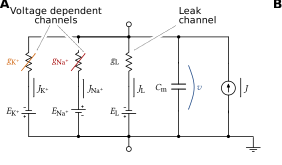
\includegraphics[scale=0.3333]{media/chapters/02_modelling/02_01/hodgkin_huxley_circuit.pdf}~~~~%
	\includegraphics{media/chapters/02_modelling/02_01/action_potentials_hh_conductances.pdf}
	{\phantomsubcaption\label{fig:action_potentials_hh_conductances_circuit}}
	{\phantomsubcaption\label{fig:action_potentials_hh_conductances_conductances}}
	\vspace{-0.5cm}
	\caption[Equivalent circuit diagram of the Hodgkin-Huxley model]{Equivalent circuit diagram of the Hodgkin-Huxley model. \textbf{(A)} Equivalent circuit model of the Hodgkin-Huxley model. The resting potential is generated by a virtual \enquote{leak} channel; the $\mathrm{K}^+$ and $\mathrm{Na}^+$ channels vary over time and depend on the membrane potential. \textbf{(B)} Conductance traces for a single action potential (slice from \cref{fig:action_potentials_superthreshold}). Sodium drives depolarisation, potassium repolarisation.}
	\label{fig:action_potentials_hh_conductances}
\end{figure}

Conveniently, Hodgkin-Huxley-type models are an extension of the equivalent cell-membrane circuit from the previous subsection (\Cref{fig:electrical_circuit}).
We just need to make two conceptual changes to account for the linear subthreshold and nonlinear superthreshold dynamics.

\subsubsection{Subthreshold dynamics}
To model the linear subthreshold dynamics, we simply add a capacitor with capacitance $C_\mathrm{m}$ to the circuit model.
This \emph{membrane capacitance}\index{neuron!membrane capacitance} is physically motivated by the cell membrane separating two electrically charged bodies.
Any such system inherently possesses capacitive properties.%
\footnote{To be clear, the membrane capacitance is not specific to the Hodgkin-Huxley model. In fact, this assumption preceded the Hodgkin-Huxley model by several decades (e.g., \cite{lapicque1907recherches}). We discuss the corresponding LIF neuron model first proposed by Lapicque later in this chapter.}
Given an input current $J(t)$, the sub-threshold dynamics can be described in terms of the following differential equation
\begin{align}
	\begin{aligned}
	\CMem \dot\vMem(t) &=
		  g_\mathrm{K^+} \bigl(E_\mathrm{K^+} - \vMem(t)\bigr)
		+ g_\mathrm{Na^+} \bigl(E_\mathrm{Na^+} - \vMem(t)\bigr)
		+ g_\mathrm{Cl^-} \bigl(E_\mathrm{Cl^-} - \vMem(t)\bigr) + J(t) \\ &=
	g_\mathrm{L} \bigl(\EL - \vMem(t)\bigr) + J(t) \,.
	\end{aligned}
\end{align}
The last term simplifies the dynamics using a \emph{leak conductance} \gL and \emph{leak potential} \EL that form a basic resistor-capacitance (RC) circuit (right half of \Cref{fig:action_potentials_hh_conductances_circuit}) with the time-constant $\tauMem = \CMem g_\mathrm{L}^{-1}$.
We have
\begin{align*}
	\gL &= g_\mathrm{K^+} + g_\mathrm{Na^+} + g_\mathrm{Cl^-} \,, &
	\text{and} \quad \quad \EL &= \frac{g_\mathrm{K^+} E_\mathrm{K^+} +
				 	g_\mathrm{Na^+} E_\mathrm{Na^+} + g_\mathrm{Cl^-} E_\mathrm{Cl^-}}{g_\mathrm{K^+} + g_\mathrm{Na^+} + g_\mathrm{Cl^-}} \,.
\end{align*}
The equation for \EL is exactly the equilibrium potential as per \cref{eqn:circuit_equilibrium_ions}.
In the absence of an input current $J(t)$, \EL is a stable attractor in the subtreshold dynamics.
It typically holds $\vRest = \EL$; still, we use \EL in this context to emphasise its use as a conductance-based channel.

\subsubsection{Superthreshold dynamics}
The superthreshold dynamics are responsible for action potential generation.
We describe these nonlinear dynamics in terms of potassium and sodium channels with time-dependent conductances $g_\mathrm{K^+}(t)$, $g_\mathrm{Na^+}(t)$ (\Cref{fig:action_potentials_hh_conductances_circuit}):
\begin{align*}
	\CMem \dot\vMem(t) &=
		  g_\mathrm{K^+}(t) \bigl(E_\mathrm{K^+} - \vMem(t)\bigr)
		+ g_\mathrm{Na^+}(t) \bigl(E_\mathrm{Na^+} - \vMem(t)\bigr)
		+ g_\mathrm{L} \bigl(\EL - \vMem(t)\bigr) + J(t) \,.
\end{align*}
Hodgkin and Huxley define the time-course of these conductances in terms of a dynamical system of gating variables $m(t)$, $h(t)$, and $n(t) \in [0, 1]$ that in turn depend on $\vMem(t)$.
We have
\begin{align*}
	g_\mathrm{K^+}(t) &= \hat g_\mathrm{K^+} n(t)^4 \,, &
	g_\mathrm{Na^+}(t) &= \hat g_\mathrm{Na^+} m(t)^3 h(t) \,,
\end{align*}
where $\hat g_\mathrm{K^+}$ and $\hat g_\mathrm{Na^+}$ are the maximum conductances.
%Using place-holder functions $f_m$, $f_n$, $f_h$, the dynamics of the gating variables are
%\begin{align*}
%	\dot m(t) &= f_m(v(t), m(t)) \,, &
%	\dot h(t) &= f_h(v(t), h(t)) \,, &
%	\dot n(t) &= f_n(v(t), n(t)) \,.
%\end{align*}
The dynamics of the gating variables (cf.~\Cref{app:hippocampal_hh}) produce a tight feedback loop between $\vMem(t)$ and the conductances.

\Cref{fig:action_potentials_hh_conductances_conductances} depicts the resulting conductances over time.
In particular, $g_\mathrm{Na^+}(t)$ rises rapidly once a certain threshold potential is exceeded.
This drives the cell towards the positive sodium reversal potential $E_\mathrm{Na^+}$; the cell becomes depolarised.
In turn, the positive membrane potential triggers a rise in potassium conductivity $g_\mathrm{K^+}(t)$, while the gating variable $h(t)$ shuts the sodium current off. This drives the cell towards the negative potassium reversal potential $E_\mathrm{K^+}$; the cell becomes hyperpolarised, while the potassium conductance remains relatively high for a short time.
This accounts for refractoriness, as large $J$ are required to counter the potassium current.

A detailed description of the superthreshold dynamics is provided in \Cref{app:hippocampal_hh}, including the unabridged equations and additional diagrams.
An even more thorough discussion of the dynamics of Hodgkin-Huxley-like neurons may be found in \citet{izhikevich2007dynamical}.

\subsection{Compartmental Neuron Models}
\label{sec:comp}

\begin{figure}
	\centering
	\includegraphics{media/chapters/02_modelling/02_01/compartments.pdf}
	{\phantomsubcaption\label{fig:compartments_physical}}%
	{\phantomsubcaption\label{fig:compartments_volumes}}%
	{\phantomsubcaption\label{fig:compartments_circuit}}%
	\caption[Equivalent circuit of an exemplary compartmental neuron model]{Equivalent circuit diagram of an exemplary compartmental neuron model. \textbf{(A)} A biological neuron is divided into $N = 6$ individual compartments (neuron redrawn from \cite{howell1916textbook}, Figure~84, p.~187).
	\textbf{(B)} Compartments are often approximated as cylinders; using \enquote{cable theory} one can compute how potentials propagate along the membrane.
	\textbf{(C)} Cylinder models can be further simplified by modelling each compartment as a simple equivalent circuit. Here, the somatic compartment (orange) possesses Hodgkin-Huxley-like voltage-dependent dynamics. Individual model circuits are resistively coupled with conductances $g_{ij}$.
	}
	\label{fig:compartments}
\end{figure}

As we saw at the beginning of this section, neurons possess intricate morphologies (cf.~\Cref{fig:compartments_physical}).
Up to this point, we have minimised this fact and instead summarised neural electrophysiology in terms of a single membrane potential over time, $\vMem(t)$.
Models based on this assumption are referred to as \emph{point neurons} or \emph{single compartment models}.

As we discuss in more detail in \Cref{chp:nlif}, the spatial organization of a neuron can have a significant impact on its function.
This is because the intracellular fluid is not a particularly good electrical conductor.
Combined with the capacitive properties of the membrane, we can, at a single point in time, measure different membrane potentials throughout the neuron.
These voltage differences cause currents injected at different points of the neuron to interact nonlinearly, which supports computation.
Perhaps confusingly, the neural \emph{dynamics} we describe here are mostly linear, but the \emph{average effect over time} is nonlinear.

\begin{figure}
	\includegraphics{media/chapters/02_modelling/02_01/cylinder.pdf}
	\caption[Illustration of potential propagation within a cylindrical cable.]{Illustration of potential propagation within a cylindrical cable. Injecting a \SI{1}{\nano\ampere} current at the centre of a \SI{1}{\milli\metre} long cable (diameter \SI{1}{\micro\metre}, capacitance \SI{1}{\micro\farad\per\square\centi\metre}, longitudinal resistance \SI{150}{\ohm\per\centi\metre}, leak conductance \SI{0.5}{\milli\siemens\per\square\centi\metre}). \textbf{(A)} Potential at different points $x$ and times $t$ (see \emph{(B)} for a legend) in a linear cable. \textbf{(B)} Continuous representation of the same data; see \emph{(A)} for the mapping between colours and voltages.}
	\label{fig:cylinder}
\end{figure}

A quite faithful model of this can be constructed using \emph{cable theory}.
To this end, individual neurons are approximated as an arrangement of cylinders that represent individual segments of the neuron (\Cref{fig:compartments_volumes}).
Voltages spatially propagate through these cylinders. That is, the model takes the longitudinal resistance of the individual neuron segments as well as their capacitative properties into account.
Given an input impulse, we can use \emph{cable equations} to predict the voltage $v(x, t)$ at a certain position $x$ along the segment at a time $t$ (cf.~\Cref{fig:cylinder}).
Mathematically, this can be accomplished by assuming an infinite number of resistively coupled RC circuits and solving a partial differential equation \citep[Chapter~2]{koch1999biophysics}.


Instead of modelling spatial propagation of voltages through cylinders, individual cylinders can be approximated as one or multiple instances of the underlying equivalent circuit.
Each of these instances is referred to as a \emph{compartment} (\Cref{fig:compartments_circuit}).
Such neuron models are correspondingly called \emph{multi-compartment} or \emph{compartmental} neuron models.
In theory, the number of compartments $N$ determines how closely the model can be made to match empirical data---some detailed neuron models rely on thousands of individual segments.
However, for most network-level research, compartments can often be joined into reduced models that capture most of the original neural behaviour \citep{herz2006modeling}.

Depending on the modelling assumptions, compartments may either be \emph{active} or \emph{passive}.
Active compartments---such as the \enquote{somatic} compartment in \Cref{fig:compartments_circuit}---model superthreshold dynamics and are capable of producing spikes, for example by including voltage-dependent Hodgkin-Huxley type models.
In contrast, passive compartments are typically modelled as the simple linear subthreshold RC-circuit.
A more detailed description of such models, including the passive dendritic trees we discuss later, can be found in \citet[Chapter~3]{koch1999biophysics} and \citet[Chapter~2]{gerstner2002spiking}.

If we assume that individual neural compartments are resistively coupled, the current $J_i(t)$ flowing into the $i$th compartment is, according to Kirchhoff's circuit laws, given as
\begin{align}
	J_i(t) &= \sum_{j = 1}^N c_{ij} \bigl(v_j(t) - v_i(t)\bigr) \,.
	\label{eqn:multi_comp_current}
\end{align}
Here, $c_{ij} = c_{ji}$ is the conductance between the $i$th and $j$th compartment. A value of $c_{ij} = 0$ indicates no connection.
Mathematically, the conductances $c_{ij}$ correspond to the symmetric adjacency matrix of an undirected connectivity graph describing the compartmental model.
